\chapter{जीन अभिव्यक्ति का नियंत्रण}\label{ch:b1:expression-control}

ग्लूकोज़ पर बढ़ता कोई जीवाणु उस \omterm{def:b1:enzymes:enzyme}{एंजाइम} के पाँच अणु ढोता है जो लैक्टोस
पचाता है; उसे लैक्टोस दीजिए और मिनटों के भीतर वह पाँच हज़ार ढोने लगता
है। किसी यकृत \omterm{def:b1:cell-unit-of-life:cell}{कोशिका} और किसी \omterm{def:b1:body-plans-tissues:nervous}{न्यूरॉन} के पास वही बीस हज़ार \omterm{def:b1:genomes:gene}{जीन} हैं और वे
लगभग पूरी तरह अलग-अलग प्रोटीन-समुच्चय बनाते हैं, और कोई भी दूसरे वाले
कभी नहीं बनाएगा। \cref{ch:b1:gene-expression} में इसकी कोई व्याख्या नहीं:
अभिव्यक्ति की मशीनरी हर \omterm{def:b1:genomes:gene}{जीन} के लिए वही है। जो भिन्न है वह यह है कि कोई
\omterm{def:b1:genomes:gene}{जीन} पढ़ा जाता है या नहीं, कितनी बार, और कितनी देर तक --- और ये निर्णय
उन्नायक पर \omterm{def:b1:nucleic-acids:chain}{DNA} बाँधते \omterm{def:b1:proteins:peptide}{प्रोटीन} लेते हैं, तथा उसके बाद संदेशवाहक और \omterm{def:b1:proteins:peptide}{प्रोटीन}
की नियति। यह अध्याय बताता है कि जीवाणु अपने भोजन के अनुसार \omterm{def:b1:genomes:gene}{जीन} कैसे चालू
और बंद करते हैं, \omterm{def:b1:cell-unit-of-life:prokeuk}{सुकेंद्रकी} अपने \omterm{def:b1:genomes:gene}{जीन} क्रोमैटिन, दूर के \omterm{def:b1:expression-control:enhancer}{संवर्धकों} और कारकों
के संयोजनों से कैसे नियंत्रित करते हैं, और वही नियंत्रण, अलग-अलग
\omterm{def:b1:cell-unit-of-life:cell}{कोशिकाओं} में अलग-अलग \omterm{def:b1:genomes:gene}{जीनों} पर लागू होकर, एक ही \omterm{def:b1:genomes:genome}{जीनोम} से शरीर कैसे बना
देता है।

\section{जीन क्यों और कहाँ नियंत्रित होते हैं}

\begin{proposition}[अभिव्यक्ति हर स्तर पर नियमित होती है]\label{prop:b1:expression-control:levels}
\index{जीन नियमन}\index{सतत जीन}
कुछ \omterm{def:b1:genomes:gene}{जीन} \emph{सतत} हैं --- यानी सदा, एक स्थिर स्तर पर अभिव्यक्त, क्योंकि
उनके उत्पाद सदा चाहिए (\omterm{def:b1:gene-expression:ribosome}{राइबोसोम} के \omterm{def:b1:proteins:peptide}{प्रोटीन}, \omterm{def:b1:respiration-fermentation:glycolysis}{ग्लाइकोलिसिस} के \omterm{def:b1:enzymes:enzyme}{एंजाइम})।
अधिकांश \emph{नियमित} हैं: यानी केवल कुछ परिस्थितियों में, कुछ \omterm{def:b1:cell-unit-of-life:cell}{कोशिकाओं}
में, कुछ क्षणों पर अभिव्यक्त। नियंत्रण इस प्रवाह के हर चरण पर काम करता है
--- मुख्यतः अनुलेखन के आरंभ पर, जो निर्णय लेने की सबसे सस्ती जगह है, पर
संदेशवाहक के प्रसंस्करण, निर्यात, स्थायित्व तथा अनुवादन पर भी, और
\omterm{def:b1:proteins:peptide}{प्रोटीन} के रूपांतरण तथा तोड़े जाने पर भी --- और अनुक्रिया-काल सेकंडों
(कोई \omterm{def:b1:proteins:peptide}{प्रोटीन} रूपांतरित) से लेकर मिनटों (कोई जीवाणु \omterm{def:b1:genomes:gene}{जीन} चालू) से होते हुए
दिनों (कोई क्रोमैटिन अवस्था बदली) तक फैले हैं।
\end{proposition}

\begin{example}[एंजाइम केवल तभी बनाना जब चाहिए]\label{ex:b1:expression-control:economy}
\omterm{def:b1:enzymes:enzyme}{एंजाइम} $\beta$-गैलैक्टोसिडेज़, जो लैक्टोस तोड़ता है, \qty{1024}{}
अवशेषों की चार शृंखलाओं का चतुष्क है: पाँच हज़ार प्रतियाँ \omterm{def:b1:cell-unit-of-life:cell}{कोशिका} के
\omterm{def:b1:proteins:peptide}{प्रोटीन} का \qty{3}{\%} हैं और प्रति पीढ़ी \qty{8e7}{} \omterm{def:b1:water-small-molecules:atp}{ATP} की क़ीमत की।
जो जीवाणु उन्हें बिना किसी लैक्टोस के बनाए वह उस स्पर्धी से लगभग एक
प्रतिशत धीमे बढ़ेगा जो नहीं बनाता, और कुछ सौ पीढ़ियों में संख्या में पिछड़
जाएगा। नियमन इसीलिए चुना गया है कि अभिव्यक्ति महँगी है।
\end{example}

\section{lac ऑपेरॉन}

\begin{definition}[ऑपेरॉन, दमनकारी, प्रचालक]\label{def:b1:expression-control:operon}
\index{ऑपेरॉन}\index{दमनकारी}\index{प्रचालक}\index{lac ऑपेरॉन}
\emph{ऑपेरॉन} जीवाणु \omterm{def:b1:genomes:gene}{जीनों} का वह समूह है जो एक ही उन्नायक से एक ही
संदेशवाहक में साथ अनुलेखित होता है, और इसलिए साथ ही नियंत्रित भी। \emph{E. coli}
का \emph{lac ऑपेरॉन} लैक्टोस के उपयोग के तीन \omterm{def:b1:genomes:gene}{जीनों} का है
--- \emph{lacZ} ($\beta$-गैलैक्टोसिडेज़), \emph{lacY} (वह
लैक्टोस पारगमक जो उसे भीतर लाता है) और \emph{lacA} --- जो किसी
उन्नायक और किसी \emph{प्रचालक} के पीछे हैं, यानी उस छोटे अनुक्रम के जो
उन्नायक से अतिव्यापी है। एक अलग \omterm{def:b1:genomes:gene}{जीन}, \emph{lacI}, \emph{lac
दमनकारी} बनाता है, यानी वह \omterm{def:b1:proteins:peptide}{प्रोटीन} जो प्रचालक से बँधकर पॉलिमरेज़ को रोक
देता है। लैक्टोस, जो \omterm{def:b1:cell-unit-of-life:cell}{कोशिका} में ऐलोलैक्टोस में बदल जाता है,
\emph{प्रेरक} है: वह दमनकारी से बँधता है, उसकी आकृति बदल देता है, और
उससे प्रचालक छुड़वा देता है। इस तरह ऑपेरॉन तब तक बंद रहता है जब तक
लैक्टोस न हो --- यानी \emph{ऋणात्मक नियंत्रण} जिसे \emph{प्रेरण} हटाता
है।
\end{definition}

\begin{omfigure}
\begin{tikzpicture}[font=\footnotesize, >=Stealth, line cap=round]
  % state 1: no lactose
  \begin{scope}
    \draw[very thick, gray] (0,0) -- (11,0);
    \fill[omExo!50] (0.2,-0.2) rectangle (1.6,0.2); \node[anchor=south, font=\scriptsize] at (0.9,0.25) {\emph{lacI}};
    \fill[omProp!50] (2.4,-0.2) rectangle (3.6,0.2); \node[anchor=north, font=\scriptsize] at (3.0,-0.25) {उन्नायक};
    \fill[omThm!50] (3.6,-0.2) rectangle (4.4,0.2); \node[anchor=south, font=\scriptsize] at (4.0,0.25) {प्रचालक};
    \fill[omDef!60] (4.5,-0.2) rectangle (7.2,0.2); \node[anchor=south, font=\scriptsize] at (5.85,0.25) {\emph{lacZ}};
    \fill[omDef!60] (7.3,-0.2) rectangle (9.0,0.2); \node[anchor=south, font=\scriptsize] at (8.15,0.25) {\emph{lacY}};
    \fill[omDef!60] (9.1,-0.2) rectangle (10.3,0.2); \node[anchor=south, font=\scriptsize] at (9.7,0.25) {\emph{lacA}};
    \node[draw, thick, fill=omThm!25, rounded corners=3pt, inner sep=2pt] (rep) at (4.0,-0.95) {दमनकारी};
    \draw[->, thick] (0.9,-0.25) -- (0.9,-0.95) -- (3.3,-0.95);
    \draw[thick] (rep) -- (4.0,-0.22);
    \node[draw, thick, fill=omProp!25, rounded corners=3pt, inner sep=2pt] at (2.2,0.9) {RNA पॉलिमरेज़};
    \node[font=\scriptsize, anchor=west] at (3.45,0.9) {रुका हुआ};
    \node[anchor=east, align=right] at (-0.2,0) {लैक्टोस नहीं:\\ ऑपेरॉन बंद};
  \end{scope}
  % state 2: lactose present
  \begin{scope}[yshift=-3.0cm]
    \draw[very thick, gray] (0,0) -- (11,0);
    \fill[omExo!50] (0.2,-0.2) rectangle (1.6,0.2);
    \fill[omProp!50] (2.4,-0.2) rectangle (3.6,0.2);
    \fill[omThm!50] (3.6,-0.2) rectangle (4.4,0.2);
    \fill[omDef!60] (4.5,-0.2) rectangle (7.2,0.2); \fill[omDef!60] (7.3,-0.2) rectangle (9.0,0.2); \fill[omDef!60] (9.1,-0.2) rectangle (10.3,0.2);
    \node[draw, thick, fill=omThm!25, rounded corners=3pt, inner sep=2pt] (rep2) at (4.0,-1.0) {दमनकारी + प्रेरक};
    \node[font=\scriptsize, anchor=west] at (5.6,-1.0) {प्रचालक से छूटा हुआ};
    \node[draw, thick, fill=omProp!25, rounded corners=3pt, inner sep=2pt] at (3.0,0.85) {RNA पॉलिमरेज़};
    \draw[->, very thick, omProp!80!black] (4.0,0.85) -- (10.3,0.85) node[midway, above, font=\scriptsize] {तीनों जीनों के लिए एक ही संदेशवाहक};
    \node[anchor=east, align=right] at (-0.2,0) {लैक्टोस मौजूद:\\ ऑपेरॉन चालू};
  \end{scope}
\end{tikzpicture}

{\small \omterm{def:b1:expression-control:operon}{lac ऑपेरॉन}। लैक्टोस के बिना \omterm{def:b1:expression-control:operon}{दमनकारी} \omterm{def:b1:expression-control:operon}{प्रचालक} पर बैठा रहता है और
पॉलिमरेज़ शुरू नहीं हो पाता; और लैक्टोस के साथ प्रेरक \omterm{def:b1:expression-control:operon}{दमनकारी} को खींच
लेता है तथा तीनों \omterm{def:b1:genomes:gene}{जीन} एक ही संदेशवाहक में अनुलेखित हो जाते हैं।}
\end{omfigure}

\begin{proposition}[ऑपेरॉन मॉडल]\label{prop:b1:expression-control:jacobmonod}
lac \omterm{def:b1:genomes:gene}{जीन} किसी विसरणशील \omterm{def:b1:expression-control:operon}{दमनकारी} से नियंत्रित होते हैं जो \omterm{def:b1:genomes:gene}{जीनों} से सटे किसी
स्थल पर काम करता है: नियंत्रण ऋणात्मक है, \omterm{def:b1:expression-control:operon}{दमनकारी} \emph{ट्रांस} में
(\omterm{def:b1:cell-unit-of-life:cell}{कोशिका} में कहीं से भी) काम करता है, और \omterm{def:b1:expression-control:operon}{प्रचालक} \emph{सिस} में
(केवल अपने बग़ल के \omterm{def:b1:genomes:gene}{जीनों} पर)।
\end{proposition}
\begin{proof}[साक्ष्य]
याकोब और मोनो (1959--1961) ने उत्परिवर्तियों से तर्क किया।
\emph{lacI} में उत्परिवर्ती नस्लें ($I^-$) लैक्टोस के साथ भी और बिना भी
\omterm{def:b1:enzymes:enzyme}{एंजाइम} बनाती थीं (\emph{सतत}); और उस क्षेत्र की किसी दूसरी प्रति पर लाया
गया सामान्य \emph{lacI} \omterm{prop:b1:expression-control:levels}{जीन नियमन} लौटा देता था, इसलिए उस \omterm{def:b1:genomes:gene}{जीन} का उत्पाद
कोई विसरणशील \omterm{def:b1:expression-control:operon}{दमनकारी} है जो उत्परिवर्ती में नहीं होता। \omterm{def:b1:expression-control:operon}{प्रचालक} में
उत्परिवर्ती नस्लें ($O^c$) भी सतत थीं, पर किसी दूसरी प्रति पर का कोई
सामान्य \omterm{def:b1:expression-control:operon}{प्रचालक} नियमन नहीं लौटाता था --- \omterm{def:b1:expression-control:operon}{प्रचालक} केवल उन्हीं \omterm{def:b1:genomes:gene}{जीनों} को
नियंत्रित करता है जो उससे भौतिक रूप से जुड़े हों, इसलिए वह कोई स्थल है,
कोई उत्पाद नहीं। एक तीसरा वर्ग ($I^s$) बिलकुल प्रेरित नहीं हो पाता था
और प्रभावी था: यानी ऐसा \omterm{def:b1:expression-control:operon}{दमनकारी} जो अब प्रेरक को बाँधता नहीं। PaJaMo
प्रयोग (1959) में संयुग्मन से किसी $I^-$ \omterm{def:b1:cell-unit-of-life:cell}{कोशिका} में पहुँचाया गया कोई
सामान्य \emph{lacI} \omterm{def:b1:genomes:gene}{जीन} मिनटों के भीतर एंजाइम-संश्लेषण बंद कर देता था:
यानी \omterm{def:b1:expression-control:operon}{दमनकारी} तेज़ी से, और अनुलेखन पर काम करता है --- और बाद में दिखाया
गया कि संदेशवाहक का अर्ध-आयु कुछ ही मिनट है।
\end{proof}

\begin{definition}[धनात्मक नियंत्रण: CAP और चक्रीय AMP]\label{def:b1:expression-control:cap}
\index{अपचयज दमन}\index{द्विवृद्धि}
lac उन्नायक कमज़ोर है: \omterm{def:b1:expression-control:operon}{दमनकारी} के बिना भी पॉलिमरेज़ कम ही शुरू होता है,
जब तक कोई दूसरा \omterm{def:b1:proteins:peptide}{प्रोटीन}, \emph{CAP} (अपचयज सक्रियक
\omterm{def:b1:proteins:peptide}{प्रोटीन}), उससे ठीक ऊपर-प्रवाह बँधकर \omterm{def:b1:nucleic-acids:chain}{DNA} को मोड़ न दे और पॉलिमरेज़ को अपनी
जगह थाम न ले। CAP \omterm{def:b1:nucleic-acids:chain}{DNA} से केवल तभी बँधता है जब वह
\emph{चक्रीय AMP} ढो रहा हो, जिसका \omterm{def:b1:cell-unit-of-life:cell}{कोशिका} में स्तर ग्लूकोज़ प्रचुर होने
पर गिर जाता है। इसलिए \omterm{def:b1:expression-control:operon}{ऑपेरॉन} पूरी तरह तभी चालू होता है जब लैक्टोस मौजूद
हो \emph{और} ग्लूकोज़ अनुपस्थित: यानी दो संकेत, एक ऋणात्मक और एक
धनात्मक, एक ही उन्नायक पर समाकलित होते हैं। दोनों शर्कराएँ मिलने पर
\emph{E. coli} पहले ग्लूकोज़ खाता है, फिर रुकता है जबकि चक्रीय AMP चढ़ता
है और lac \omterm{def:b1:enzymes:enzyme}{एंजाइम} बनते हैं, और फिर लैक्टोस खाता है --- यानी दो-चरणी
वृद्धि वक्र, जिसे \emph{द्विवृद्धि} कहते हैं, और जिसका वर्णन मोनो ने 1941
में किया तथा जिसने उन्हें \omterm{def:b1:expression-control:operon}{ऑपेरॉन} के रास्ते पर लगा दिया।
\end{definition}

\begin{omfigure}
\begin{tikzpicture}
\begin{semilogyaxis}[
  width=0.86\linewidth, height=6.0cm,
  axis x line=bottom, axis y line=left,
  xmin=0, xmax=6, ymin=1e7, ymax=3e9,
  xlabel={समय (h)}, ylabel={प्रति mL कोशिकाएँ},
  xlabel style={font=\small, at={(axis description cs:0.5,-0.12)}, anchor=north},
  ylabel style={font=\small},
  tick label style={font=\small}, xtick={0,1,2,3,4,5,6},
  clip=false,
]
\addplot[very thick, omDef, domain=0:2, samples=30] {1e7*2^(x/0.333)};
\addplot[very thick, omDef, domain=2:2.6, samples=5] {6.4e8};
\addplot[very thick, omDef, domain=2.6:4.0, samples=30] {6.4e8*2^((x-2.6)/0.5)};
\addplot[very thick, omDef, domain=4.0:6, samples=5] {6.4e8*2^(1.4/0.5)};
\node[font=\scriptsize, anchor=north west, align=left] at (axis cs:0.15,8e8) {चरण 1: ग्लूकोज़\\ (दुगुनन \qty{20}{min})};
\node[font=\scriptsize, anchor=south, align=center] at (axis cs:2.3,7e8) {ठहराव: चक्रीय AMP चढ़ता,\\ lac एंजाइम बनते};
\node[font=\scriptsize, anchor=north west, align=left] at (axis cs:3.0,9e8) {चरण 2: लैक्टोस\\ (दुगुनन \qty{30}{min})};
\node[font=\scriptsize, anchor=south west] at (axis cs:4.1,4.4e9) {};
\end{semilogyaxis}
\end{tikzpicture}

{\small ग्लूकोज़ और लैक्टोस पर \emph{E. coli} की \omterm{def:b1:expression-control:cap}{द्विवृद्धि}।
संवर्धन अकेले ग्लूकोज़ पर बढ़ता है, उसके चुकते ही रुक जाता है, और
\omterm{def:b1:expression-control:operon}{lac ऑपेरॉन} के प्रेरण में लगने वाले आधे घंटे बाद लैक्टोस पर फिर शुरू हो
जाता है।}
\end{omfigure}

\begin{omfigure}
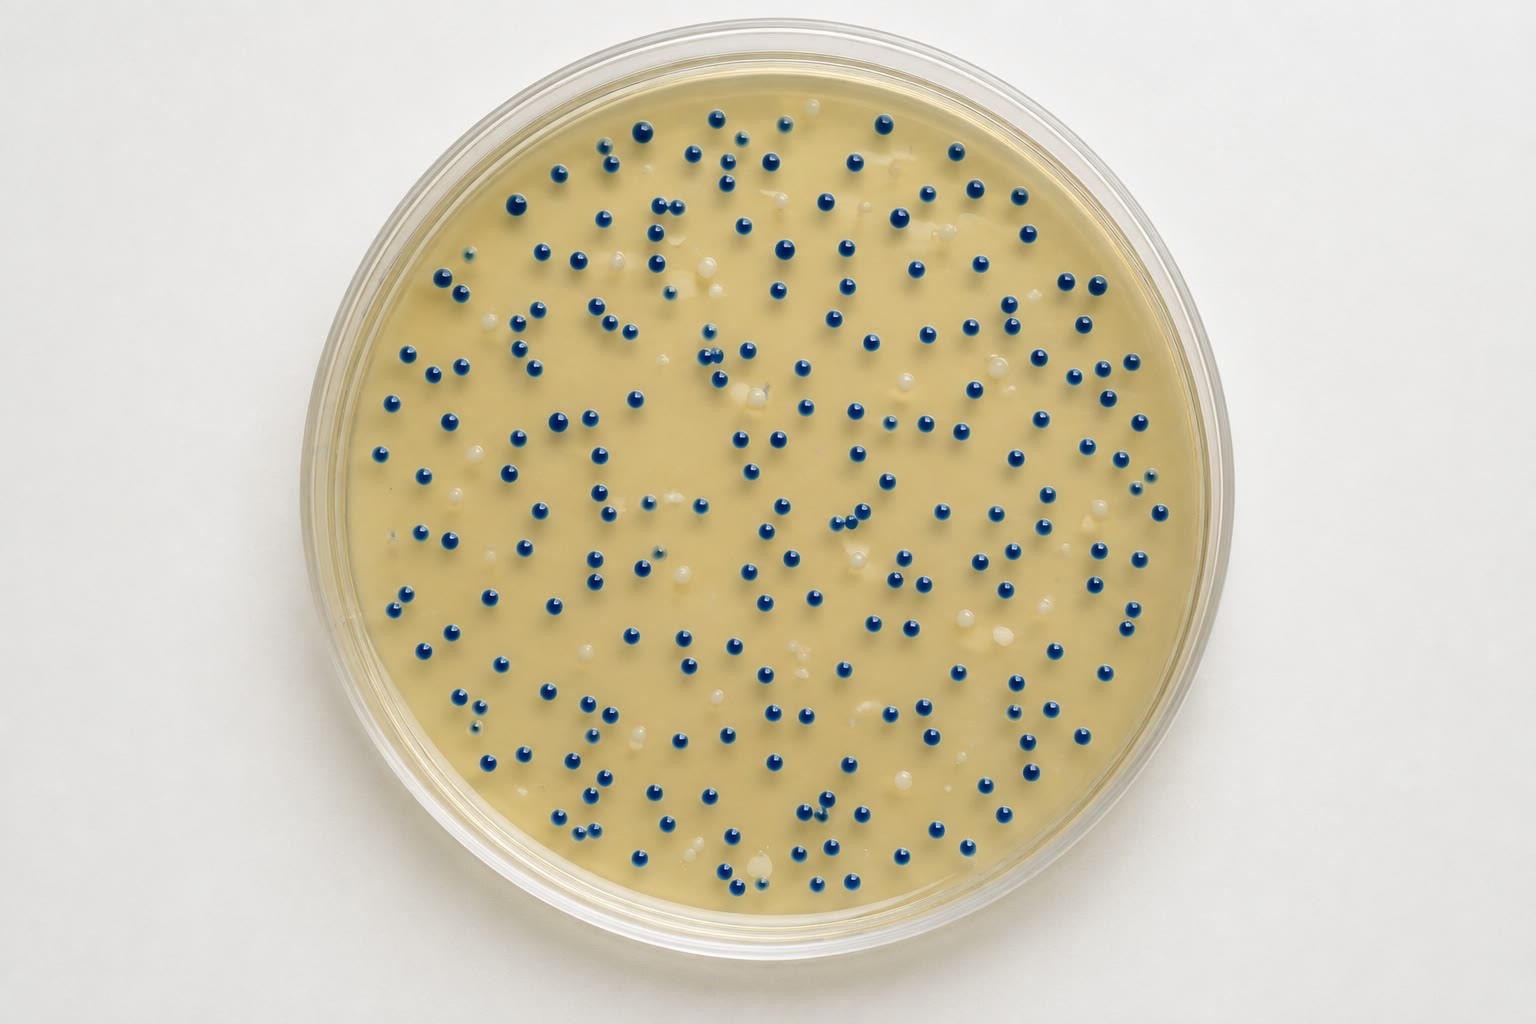
\includegraphics[width=0.46\linewidth]{images/book3/ai/b3-20-xgal-plate.jpg}

{\small दिखाई देता \omterm{def:b1:expression-control:operon}{lac ऑपेरॉन}: X-gal वाली किसी प्लेट पर उपनिवेश, जो
एक रंगहीन \omterm{def:b1:enzymes:enzyme}{क्रियाधार} है और जिसे $\beta$-गैलैक्टोसिडेज़ नीला कर देता है।
नीले उपनिवेश \emph{lacZ} अभिव्यक्त करते हैं; और सफ़ेद वाले टूटा हुआ \omterm{def:b1:genomes:gene}{जीन}
ढोते हैं --- यही वह संसूचक है जो हज़ार प्रयोगों में काम आया।}
\end{omfigure}

\begin{method}[किसी lac लक्षणप्ररूप की भविष्यवाणी]\label{met:b1:expression-control:lacphenotype}
\begin{enumerate}
  \item उस क्षेत्र की हर प्रति का जीनप्ररूप लिखिए: $I$, $P$, $O$,
        $Z$ ($^+$ सामान्य, $^-$ निष्क्रिय, $O^c$ प्रचालक-सतत,
        $I^s$ अति-दमनकारी)।
  \item \omterm{def:b1:expression-control:operon}{दमनकारी} ट्रांस में काम करता है: कहीं भी एक $I^+$ हर सामान्य
        \omterm{def:b1:expression-control:operon}{प्रचालक} का दमन करता है; और $I^s$ प्रेरक कुछ भी हो, दमन करता है।
  \item \omterm{def:b1:expression-control:operon}{प्रचालक} और उन्नायक सिस में काम करते हैं: कोई $O^c$ केवल अपने ही
        \omterm{def:b1:nucleic-acids:chain}{DNA} का $Z$ मुक्त करता है; और कोई $P^-$ केवल अपने ही \omterm{def:b1:genomes:gene}{जीन} चुप
        करता है।
  \item प्रेरक के साथ और उसके बिना पूछिए कि हर $Z^+$ \omterm{def:b1:genomes:gene}{जीन} अनुलेखित होता
        है या नहीं; उसी के अनुसार लक्षणप्ररूप प्रेरणीय, सतत या
        अप्रेरणीय है। फिर ग्लूकोज़ जोड़िए: चक्रीय AMP और CAP के बिना
        \omterm{def:b1:expression-control:operon}{दमनकारी} चाहे कुछ भी करे, अनुलेखन कम ही रहता है।
\end{enumerate}
\end{method}

\begin{example}[दो आंशिक द्विगुणित]\label{ex:b1:expression-control:diploids}
$I^-\,O^+\,Z^+ / I^+\,O^+\,Z^-$: $I^+$ प्रति वह \omterm{def:b1:expression-control:operon}{दमनकारी} बनाती है जो
$O^+$ से बँधता है, यानी $Z^+$ के बग़ल वाले से; इसलिए प्रेरणीय ---
उत्परिवर्तन की पूर्ति हो गई। $I^+\,O^c\,Z^+ / I^+\,O^+\,Z^-$: इकलौता काम करता $Z$
ऐसे \omterm{def:b1:expression-control:operon}{प्रचालक} के पीछे बैठा है जिसे \omterm{def:b1:expression-control:operon}{दमनकारी} बाँध नहीं सकता; इसलिए सतत ---
और दूसरी प्रति का सामान्य \omterm{def:b1:expression-control:operon}{प्रचालक} कुछ नहीं कर सकता, क्योंकि वह केवल टूटे
हुए $Z$ को नियंत्रित करता है।
\end{example}

\section{जीवाणुओं की दूसरी नीतियाँ}

\begin{proposition}[दमन, अनुक्षीणन और सिग्मा कारक]\label{prop:b1:expression-control:trp}
\index{trp ऑपेरॉन}\index{अनुक्षीणन}\index{सिग्मा कारक}
जैवसंश्लेषण के \omterm{def:b1:expression-control:operon}{ऑपेरॉन} उल्टे अर्थ में नियंत्रित होते हैं:
\emph{\omterm{prop:b1:expression-control:trp}{trp ऑपेरॉन}}, यानी ट्रिप्टोफ़ैन बनाने के पाँच \omterm{def:b1:genomes:gene}{जीन}, तब तक अनुलेखित
होता है जब तक ट्रिप्टोफ़ैन मौजूद न हो --- वह \omterm{def:b1:proteins:aminoacid}{ऐमीनो अम्ल} trp
\omterm{def:b1:expression-control:operon}{दमनकारी} से बँधकर उसे \omterm{def:b1:expression-control:operon}{प्रचालक} बाँधने \emph{योग्य बना देता है} (\omterm{def:b1:expression-control:operon}{सह-दमनकारी})।
एक दूसरा, महीन नियंत्रण, \emph{अनुक्षीणन}, जीवाणुओं में अनुलेखन तथा
अनुवादन के युग्मन का उपयोग करता है: संदेशवाहक का आरंभ एक छोटे पेप्टाइड
के लिए कूट करता है जिसमें लगातार दो ट्रिप्टोफ़ैन हैं; यदि
ट्रिप्टोफ़ैन से लदा tRNA प्रचुर हो तो कोई \omterm{def:b1:gene-expression:ribosome}{राइबोसोम} उसे जल्दी अनूदित कर
देता है और पीछे का \omterm{def:b1:nucleic-acids:chain}{RNA} किसी समापक हेयरपिन में मुड़ जाता है जो पॉलिमरेज़ को
\omterm{def:b1:genomes:gene}{जीनों} से पहले ही रोक देता है; और यदि ट्रिप्टोफ़ैन कम हो तो \omterm{def:b1:gene-expression:ribosome}{राइबोसोम}
ट्रिप्टोफ़ैन \omterm{def:b1:gene-expression:code}{कोडॉनों} पर अटक जाता है और \omterm{def:b1:nucleic-acids:chain}{RNA} अलग तरह से मुड़ जाता है, जिससे
अनुलेखन चलता रहता है। जीवाणु अपने पॉलिमरेज़ की $\sigma$ उपइकाई बदलकर पूरे
जीन-समुच्चय भी बदल देते हैं: कोई ऊष्मा-आघात $\sigma$ उसे \omterm{prop:b1:proteins:denaturation}{परिचारक} \omterm{def:b1:genomes:gene}{जीनों} के
उन्नायकों पर भेजता है; और कोई बीजाणुजनन $\sigma$ बीजाणु बनने के \omterm{def:b1:genomes:gene}{जीनों} के
उन्नायकों पर।
\end{proposition}

\section{सुकेंद्रकियों में नियंत्रण}

\begin{definition}[अनुलेखन कारक, संवर्धक]\label{def:b1:expression-control:enhancer}
\index{अनुलेखन कारक}\index{संवर्धक}
\omterm{def:b1:cell-unit-of-life:prokeuk}{सुकेंद्रकियों} में पॉलिमरेज़ कभी अपने आप शुरू नहीं होता: उन्नायक पर के
सामान्य कारक (\cref{ch:b1:gene-expression}) उसे बुला लाते हैं, और
दर \emph{नियामक अनुक्रमों} से बँधे \emph{अनुलेखन कारक} तय करते हैं
--- कुछ उन्नायक के पास, और अनेक ऐसे \emph{संवर्धकों} में जो हज़ारों
\omterm{thm:b1:nucleic-acids:helix}{क्षारक युग्म} दूर, ऊपर-प्रवाह, नीचे-प्रवाह या किसी \omterm{def:b1:genomes:gene}{इंट्रॉन} में, किसी भी
अभिविन्यास में पड़े हो सकते हैं, और जो \omterm{def:b1:nucleic-acids:chain}{DNA} को \emph{फंदा} बनाकर काम करते
हैं ताकि उन पर बँधे कारक उन्नायक के संकुल को माध्यस्थ \omterm{def:b1:proteins:peptide}{प्रोटीनों} के ज़रिए
छू सकें। कोई अनुलेखन कारक खंडीय होता है: एक \emph{DNA-बंधनकारी प्रांत}
जो किसी छोटे अनुक्रम को पहचानता है (कुंडली-मोड़-कुंडली, ज़िंक अंगुली,
ल्यूसीन ज़िप कुल) और एक \emph{सक्रियण} या \emph{दमन} प्रांत जो मशीनरी
बुलाता या रोकता है। कोई \omterm{def:b1:genomes:gene}{जीन} तब पढ़ा जाता है जब कारकों का सही
\emph{संयोजन} मौजूद हो: कुछ सौ कारक, संयोजनों में, बीस हज़ार \omterm{def:b1:genomes:gene}{जीन}
नियंत्रित करते हैं।
\end{definition}

\begin{omfigure}
\begin{tikzpicture}[font=\footnotesize, >=Stealth, line cap=round]
  % DNA with enhancer far upstream, looped to promoter
  \draw[very thick, gray] (0,0) -- (2.2,0) .. controls (3.2,0) and (3.4,2.6) .. (5.0,2.6) .. controls (6.6,2.6) and (6.8,0) .. (7.8,0) -- (12.5,0);
  \fill[omExo!60] (0.4,-0.2) rectangle (2.0,0.2); \node[anchor=north, font=\scriptsize] at (1.2,-0.25) {संवर्धक (\qtyrange{1}{100}{kb} दूर)};
  \fill[omProp!50] (8.0,-0.2) rectangle (9.4,0.2); \node[anchor=north, font=\scriptsize] at (8.7,-0.25) {उन्नायक};
  \fill[omDef!60] (9.5,-0.2) rectangle (12.3,0.2); \node[anchor=north, font=\scriptsize] at (10.9,-0.25) {जीन};
  % looped enhancer brought near promoter: draw factors at the loop apex near promoter? Simplify: activators on enhancer, mediator bridging
  \node[draw, thick, fill=omExo!30, rounded corners=3pt, inner sep=2pt] (act) at (1.2,0.75) {सक्रियक};
  \node[draw, thick, fill=omThm!25, rounded corners=3pt, inner sep=2pt, align=center] (med) at (5.0,1.5) {माध्यस्थ};
  \node[draw, thick, fill=omProp!30, rounded corners=3pt, inner sep=2pt, align=center] (pol) at (8.7,0.85) {सामान्य कारक\\ + पॉलिमरेज़};
  \draw[thick, omExo!80!black] (act) -- (2.4,1.2) -- (med);
  \draw[thick, omThm] (med) -- (pol);
  \node[anchor=north, align=center, gray] at (6.2,-1.0) {DNA फंदा बनाता है ताकि दूर बँधे कारक उन्नायक के संकुल को छू सकें;\\ कोई जीन तब पढ़ा जाता है जब कारकों का सही संयोजन बँधा हो};
\end{tikzpicture}

{\small \omterm{def:b1:expression-control:enhancer}{संवर्धक} की क्रिया। किसी दूर के \omterm{def:b1:expression-control:enhancer}{संवर्धक} से बँधे सक्रियक \omterm{def:b1:nucleic-acids:chain}{DNA} के
फंदा बनने से उन्नायक तक आ जाते हैं, और कोई माध्यस्थ संकुल उनका संकेत
पॉलिमरेज़ तक पहुँचा देता है।}
\end{omfigure}

\begin{proposition}[क्रोमैटिन भी नियंत्रण का भाग है]\label{prop:b1:expression-control:chromatin}
\index{हिस्टोन ऐसीटिलीकरण}\index{DNA मेथिलीकरण}
विषमक्रोमैटिन में जमे \omterm{def:b1:genomes:nucleosome}{न्यूक्लियोसोमों} में लिपटा कोई \omterm{def:b1:genomes:gene}{जीन} पढ़ा नहीं जा
सकता: कारक उस तक पहुँच ही नहीं पाते। सक्रियक ऐसे \omterm{def:b1:enzymes:enzyme}{एंजाइम} बुलाते हैं जो
\omterm{def:b1:genomes:nucleosome}{हिस्टोनों} का \emph{ऐसीटिलीकरण} करते हैं, जिससे \omterm{def:b1:nucleic-acids:chain}{DNA} पर उनकी पकड़ ढीली पड़
जाती है और वह क्षेत्र खुला चिह्नित हो जाता है; और \omterm{def:b1:expression-control:operon}{दमनकारी} ऐसे \omterm{def:b1:enzymes:enzyme}{एंजाइम}
बुलाते हैं जो ऐसीटिल समूह हटाते हैं और ऐसे चिह्न लगाते हैं जो क्रोमैटिन
संहत कर देते हैं। किसी उन्नायक के साइटोसीनों पर जोड़े गए मेथिल समूह उसे
टिकाऊ रूप से चुप कर देते हैं, और वे चिह्न प्रतिकृतिकरण पर नक़ल हो जाते
हैं, इसलिए किसी \omterm{def:b1:cell-unit-of-life:cell}{कोशिका} का खुले और बंद \omterm{def:b1:genomes:gene}{जीनों} का प्रतिरूप उसकी संततियों को
वंशागत होता है --- यही वह स्मृति है जिससे किसी यकृत \omterm{def:b1:cell-unit-of-life:cell}{कोशिका} की संततियाँ
यकृत \omterm{def:b1:cell-unit-of-life:cell}{कोशिकाएँ} ही रहती हैं (वर्ष 3 का खंड इन \emph{अधिजननिक}
क्रियाविधियों को विस्तार से लेता है)।
\end{proposition}
\begin{proof}[साक्ष्य]
मक्खी के डिंभकों के विशाल बहुसूत्री \omterm{def:b1:genomes:genome}{गुणसूत्रों} में (हर \omterm{def:b1:genomes:genome}{गुणसूत्र} की एक
हज़ार प्रतियाँ अगल-बगल, पट्टियों सहित) अनुलेखित हो रहे \omterm{def:b1:genomes:gene}{जीन} ऐसे
\emph{गुब्बारों} के रूप में दिखते हैं जहाँ क्रोमैटिन खुल गई है; और
हॉर्मोन इक्डाइसोन, जो निर्मोचन शुरू कराता है, मिनटों के भीतर गुब्बारों का
एक विशेष समुच्चय उभार देता है और कुछ और घंटों बाद, एक नियत क्रम में ---
यानी अनुलेखन सीधे देखा गया, और किसी संकेत से चालू हुआ। जो \omterm{def:b1:genomes:gene}{जीन}
गुणसूत्र-पुनर्व्यवस्था से विषमक्रोमैटिन के बग़ल में चले जाते हैं वे कुछ
\omterm{def:b1:cell-unit-of-life:cell}{कोशिकाओं} में चुप हो जाते हैं और कुछ में नहीं, और वह अवस्था उनकी संततियों
को वंशागत होती है।
\end{proof}

\begin{omfigure}
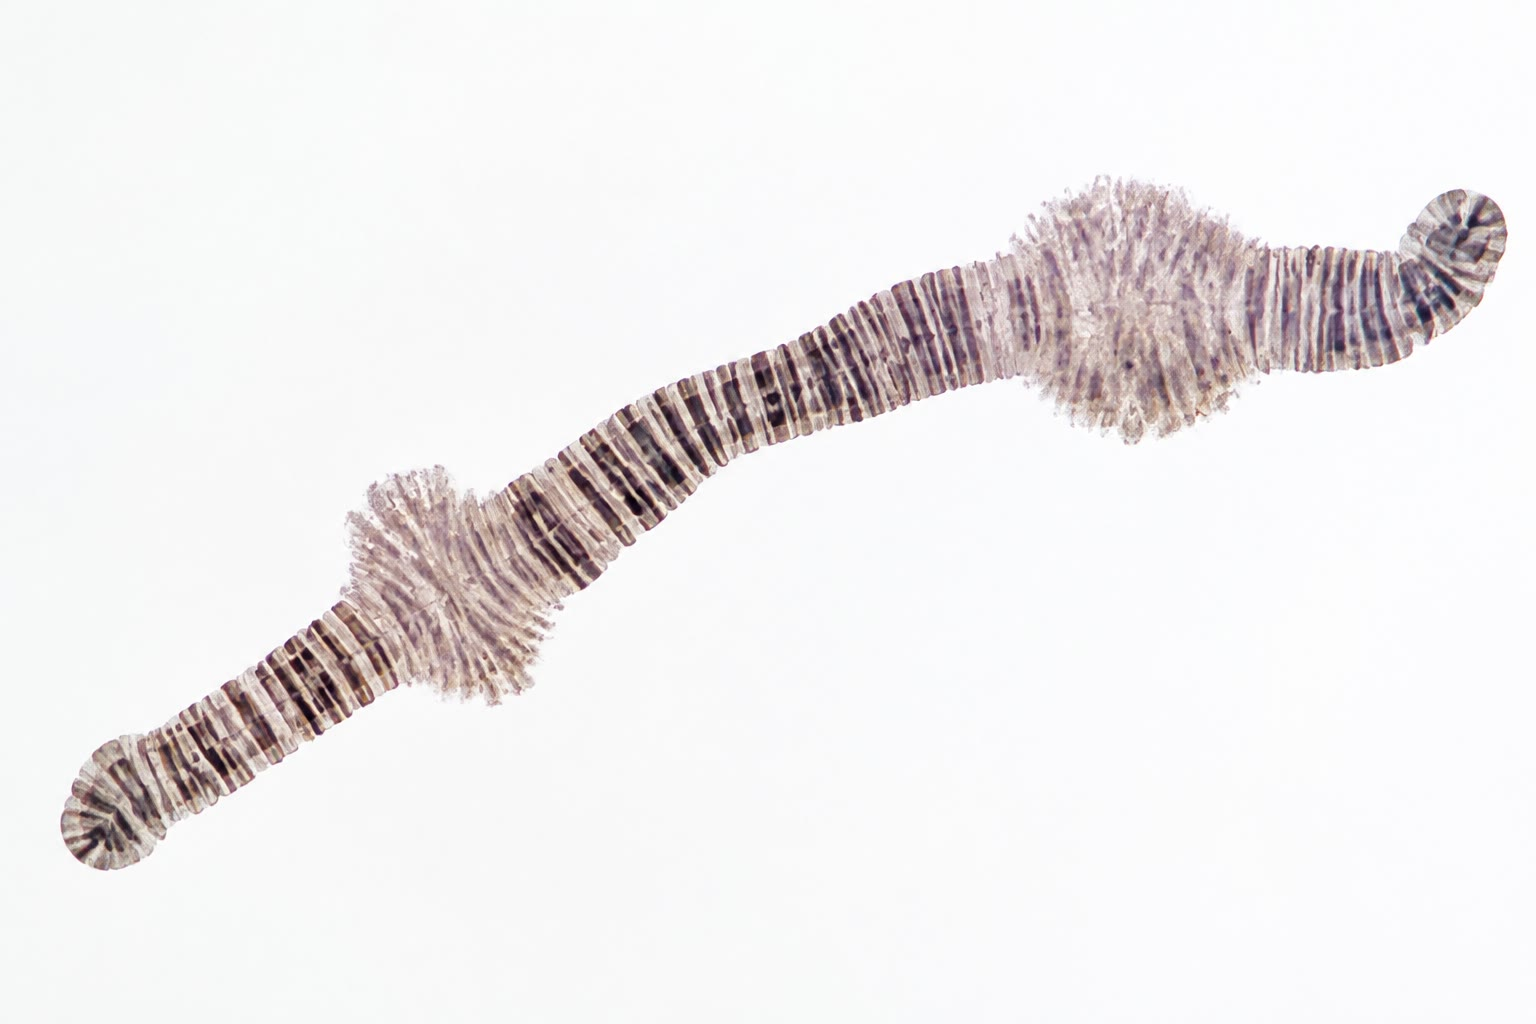
\includegraphics[width=0.56\linewidth]{images/book3/ai/b3-20-polytene-chromosome.jpg}

{\small किसी मक्खी की लार-ग्रंथि का एक बहुसूत्री \omterm{def:b1:genomes:genome}{गुणसूत्र}: पट्टीदार,
और दो गुब्बारों के साथ जहाँ क्रोमैटिन अनुलेखन के लिए खुल गई है।
गुब्बारे \omterm{def:b1:genomes:gene}{जीनों} के चालू-बंद होने के साथ उभरते और मिटते रहते हैं।}
\end{omfigure}

\begin{example}[कोई संकेत अभिव्यक्ति का प्रतिरूप बन जाता है]\label{ex:b1:expression-control:steroid}
कोर्टिसोल किसी यकृत \omterm{def:b1:cell-unit-of-life:cell}{कोशिका} में घुसता है और अपने ग्राही से बँधता है, यानी
उस \omterm{def:b1:expression-control:enhancer}{अनुलेखन कारक} से जो \omterm{def:b1:eukaryotic-cell:organelle}{कोशिकाद्रव} में निष्क्रिय रखा जाता है; वह संकुल
केंद्रक में घुसता है, सौ \omterm{def:b1:genomes:gene}{जीनों} के पास मौजूद पंद्रह-क्षारक के किसी अनुक्रम
से बँधता है --- जिनमें \omterm{def:b1:biosyntheses-integration:gluconeogenesis}{ग्लूकोजनन} के \omterm{def:b1:genomes:gene}{जीन} भी हैं (\cref{ch:b1:biosyntheses-integration}) ---
और ऐसीटिलेज़ तथा माध्यस्थ बुला लेता है: घंटे भर के भीतर
ग्लूकोज़-संश्लेषण के \omterm{def:b1:enzymes:enzyme}{एंजाइम} बनने लगते हैं। वही हॉर्मोन किसी लसीकाणु में,
जिसकी खुली क्रोमैटिन उन्हीं अनुक्रमों का कोई अलग समुच्चय उघाड़ती है,
ऐसे \omterm{def:b1:genomes:gene}{जीन} चालू कर देता है जो उस \omterm{def:b1:cell-unit-of-life:cell}{कोशिका} को मार डालते हैं। एक संकेत, एक
ग्राही, दो अनुक्रियाएँ: फ़र्क़ इसका है कि कौन-से \omterm{def:b1:genomes:gene}{जीन} पहुँच में थे।
\end{example}

\section{अनुलेखन के बाद, और शरीर का बनना}

\begin{proposition}[उन्नायक से परे नियंत्रण]\label{prop:b1:expression-control:posttranscriptional}
\index{mRNA स्थायित्व}
कोई \omterm{def:b1:cell-unit-of-life:prokeuk}{सुकेंद्रकी कोशिका} यह भी तय करती है कि कोई अनुलेख कैसे संबंधित हो
(वैकल्पिक संबंधन एक ही \omterm{def:b1:genomes:gene}{जीन} से किसी पेशी और किसी मस्तिष्क को अलग \omterm{def:b1:proteins:peptide}{प्रोटीन}
देता है), वह निर्यात हो या नहीं, कितनी देर चले (अर्ध-आयु नियामक
\omterm{def:b1:proteins:peptide}{प्रोटीनों} के संदेशों के लिए मिनटों से लेकर हीमोग्लोबिन के संदेश के लिए
दिनों तक, जिन्हें अनूदित न होने वाले क्षेत्रों के वे अनुक्रम तय करते हैं
जो \omterm{def:b1:proteins:peptide}{प्रोटीनों} तथा छोटे नियामक \omterm{def:b1:nucleic-acids:chain}{RNA} को बाँधते हैं), और वह अनूदित हो या नहीं
(लोहे से भूखी \omterm{def:b1:cell-unit-of-life:cell}{कोशिकाएँ} फ़ेरिटिन संदेश का अनुवादन उसके $5'$ सिरे से बँधे
किसी \omterm{def:b1:proteins:peptide}{प्रोटीन} से रोक देती हैं, और लोहा मौजूद होने पर उसे छोड़ देती हैं)।
\omterm{def:b1:proteins:peptide}{प्रोटीन}, एक बार बन जाने पर, रूपांतरण तथा तोड़े जाने से नियंत्रित होता है
(\cref{ch:b1:enzymes})। हर बाद का स्तर पहले वाले से तेज़ और अधिक स्थानीय
है, और अधिक महँगा भी: अनुलेखन तय करता है कि \omterm{def:b1:cell-unit-of-life:cell}{कोशिका} क्या कर सकती है, और
बाद के स्तर यह कि वह अभी क्या करती है।
\end{proposition}

\begin{proposition}[विभेदी अभिव्यक्ति शरीर बना देती है]\label{prop:b1:expression-control:differentiation}
\index{विभेदन}
किसी बहुकोशिकीय \omterm{def:b1:organism-environment:organism}{जीव} की हर \omterm{def:b1:cell-unit-of-life:cell}{कोशिका} वही \omterm{def:b1:genomes:genome}{जीनोम} ढोती है; और \omterm{def:b1:cell-unit-of-life:cell}{कोशिकाएँ} इसलिए
भिन्न हैं कि वे उसके अलग-अलग उपसमुच्चय अभिव्यक्त करती हैं।
\emph{गृहव्यवस्था} \omterm{def:b1:genomes:gene}{जीन} --- उपापचय, \omterm{def:b1:gene-expression:ribosome}{राइबोसोम} तथा \omterm{def:b1:eukaryotic-cell:cytoskeleton}{कोशिका-कंकाल} के कुछ
हज़ार --- हर \omterm{def:b1:cell-unit-of-life:cell}{कोशिका} में चालू हैं; और बाक़ी कुछ \omterm{def:b1:cell-unit-of-life:cell}{कोशिकाओं} में चालू तथा
कुछ में बंद रहते हैं, यह उन \omterm{def:b1:expression-control:enhancer}{अनुलेखन कारकों} के संयोजनों और उन क्रोमैटिन
अवस्थाओं से तय होता है जो हर \omterm{def:b1:cell-unit-of-life:cell}{कोशिका} ढोती और विरासत में पाती है। किसी लाल
\omterm{def:b1:cell-unit-of-life:cell}{कोशिका} का पूर्ववर्ती ग्लोबिन चालू कर देता है और लगभग बाक़ी सब बंद; और कोई
\omterm{def:b1:body-plans-tissues:nervous}{न्यूरॉन} अपने \omterm{def:b1:membranes-transport:transporters}{चैनल} चालू कर देता है और फिर कभी विभाजित नहीं होता।
\emph{विभेदन} अभिव्यक्ति के किसी स्थायी प्रतिरूप का पा लेना है, और
\emph{परिवर्धन} (वर्ष 2 का खंड) वह प्रक्रिया है जिससे \omterm{def:b1:cell-unit-of-life:cell}{कोशिकाओं} के बीच के
संकेत वे प्रतिरूप सही जगहों पर बिठा देते हैं।
\end{proposition}
\begin{proof}[साक्ष्य]
किसी विभेदित मेंढक \omterm{def:b1:cell-unit-of-life:cell}{कोशिका} से लिया गया केंद्रक, जब ऐसे अंडे में डाला जाए
जिसका अपना केंद्रक हटा दिया गया हो, पूरे टैडपोल का परिवर्धन चला सकता है
(गर्डन, 1962; जो लाइसेयी खंड से याद है): यानी उस विभेदित \omterm{def:b1:cell-unit-of-life:cell}{कोशिका} ने कोई
\omterm{def:b1:genomes:gene}{जीन} खोया नहीं था, केवल उन्हें बंद किया था, और अंडे के \omterm{def:b1:cell-unit-of-life:cell}{कोशिकाद्रव्य} ने वे
स्विच फिर बिठा दिए। किसी कोशिका-प्रकार के \omterm{def:b1:proteins:peptide}{प्रोटीन}, जेल पर अलग किए जाने पर,
किसी दूसरे प्रकार के \omterm{def:b1:proteins:peptide}{प्रोटीनों} से भिन्न होते हैं; उसके संदेशवाहक, अनुक्रमित
किए जाने पर, \omterm{def:b1:genomes:genome}{जीनोम} का उसी के लिए विशिष्ट उपसमुच्चय हैं; और किसी त्वचा
\omterm{def:b1:cell-unit-of-life:cell}{कोशिका} में डाले गए मुट्ठी भर \omterm{def:b1:expression-control:enhancer}{अनुलेखन कारक} उसे किसी मूल \omterm{def:b1:cell-unit-of-life:cell}{कोशिका} या किसी
\omterm{def:b1:body-plans-tissues:nervous}{न्यूरॉन} में फिर से ढाल सकते हैं।
\end{proof}

\begin{example}[दो अंगों में पढ़ा गया एक जीन]\label{ex:b1:expression-control:twoorgans}
वह \omterm{def:b1:genomes:gene}{जीन} जो ग्लूकोज़-6-फ़ॉस्फ़ेट से ग्लूकोज़ बनाने वाला \omterm{def:b1:enzymes:enzyme}{एंजाइम} देता है
केवल यकृत और गुर्दे में अभिव्यक्त होता है, और किसी दूसरे \omterm{def:b1:body-plans-tissues:tissue}{ऊतक} में नहीं:
उसका उन्नायक उन कारकों के स्थल ढोता है जो केवल वहीं मौजूद हैं, और दूसरी
\omterm{def:b1:cell-unit-of-life:cell}{कोशिकाओं} में उसका उन्नायक मेथिलित तथा उसकी क्रोमैटिन बंद रहती है। कोई
पेशी, जो उस \omterm{def:b1:genomes:gene}{जीन} को साबुत ढोती है, रक्त में ग्लूकोज़ नहीं छोड़ सकती
(\cref{ch:b1:biosyntheses-integration}) --- \omterm{def:b1:genomes:gene}{जीन} के अभाव में नहीं, बल्कि
इसलिए कि वह \omterm{def:b1:genomes:gene}{जीन} पढ़ा नहीं जाता। \omterm{def:b1:genomes:genome}{जीनोम} वही है; अभिव्यक्ति ही \omterm{def:b1:mammal-organization:organ}{अंग} है।
\end{example}

\section{अभ्यास}

\begin{exercise}[$\star$]\label{exo:b1:expression-control:1}
\omterm{def:b1:expression-control:operon}{lac ऑपेरॉन} के \omterm{def:b1:mammal-organization:organ}{अंग} बताइए और लैक्टोस के साथ तथा बिना, और ग्लूकोज़ के साथ
तथा बिना, \omterm{def:b1:expression-control:operon}{ऑपेरॉन} की अवस्था दीजिए।
\end{exercise}

\begin{exercise}[$\star$]\label{exo:b1:expression-control:2}
ट्रांस में काम करते किसी जीन-उत्पाद और सिस में काम करते किसी स्थल का
भेद समझाइए, और \omterm{def:b1:expression-control:operon}{ऑपेरॉन} से हर एक का एक उदाहरण दीजिए।
\end{exercise}

\begin{exercise}[$\star$]\label{exo:b1:expression-control:3}
\omterm{def:b1:expression-control:cap}{द्विवृद्धि} वाले आलेख से ठहराव की अवधि और हर शर्करा पर के दुगुनन-काल
पढ़िए।
\end{exercise}

\begin{exercise}[$\star$]\label{exo:b1:expression-control:4}
\omterm{def:b1:expression-control:enhancer}{संवर्धक}, \omterm{def:b1:expression-control:enhancer}{अनुलेखन कारक} और गृहव्यवस्था \omterm{def:b1:genomes:gene}{जीन} की परिभाषा दीजिए।
\end{exercise}

\begin{exercise}[$\star\star$]\label{exo:b1:expression-control:5}
इनका लक्षणप्ररूप (प्रेरणीय, सतत, अप्रेरणीय) बताइए: $I^-$;
$O^c$; $I^s$; $I^-\,O^+\,Z^+ / I^+\,O^+\,Z^+$; $I^s\,O^+\,Z^+ /
I^+\,O^+\,Z^+$; $I^+\,O^c\,Z^- / I^+\,O^+\,Z^+$।
\end{exercise}

\begin{exercise}[$\star\star$]\label{exo:b1:expression-control:6}
lac और trp \omterm{def:b1:expression-control:operon}{ऑपेरॉनों} की तुलना कीजिए: हर एक में छोटा अणु \omterm{def:b1:expression-control:operon}{दमनकारी} का क्या
करता है, और तर्क उल्टा क्यों है।
\end{exercise}

\begin{exercise}[$\star\star$]\label{exo:b1:expression-control:7}
कोई उत्परिवर्ती चक्रीय AMP नहीं बना सकता। ग्लूकोज़ पर, अकेले लैक्टोस पर,
और दोनों पर उसकी वृद्धि की, तथा हर स्थिति में
$\beta$-गैलैक्टोसिडेज़ के स्तर की भविष्यवाणी कीजिए।
\end{exercise}

\begin{exercise}[$\star\star$]\label{exo:b1:expression-control:8}
\omterm{def:b1:cell-unit-of-life:prokeuk}{सुकेंद्रकी कोशिका} की संरचना से समझाइए कि \omterm{def:b1:cell-unit-of-life:prokeuk}{सुकेंद्रकियों} में अनुक्षीणन
असंभव क्यों है।
\end{exercise}

\begin{exercise}[$\star\star$]\label{exo:b1:expression-control:9}
कोई \omterm{def:b1:expression-control:enhancer}{संवर्धक} अपने \omterm{def:b1:genomes:gene}{जीन} से \qty{5}{kb} ऊपर-प्रवाह से हटाकर
\qty{5}{kb} नीचे-प्रवाह रखा और उलट दिया जाता है; फिर भी \omterm{def:b1:genomes:gene}{जीन} अभिव्यक्त
होता है। समझाइए कि इससे \omterm{def:b1:expression-control:enhancer}{संवर्धकों} के काम करने के ढंग के बारे में क्या
पता चलता है।
\end{exercise}

\begin{exercise}[$\star\star\star$]\label{exo:b1:expression-control:10}
\qty{4096}{} अवशेषों के पाँच हज़ार $\beta$-गैलैक्टोसिडेज़ चतुष्क कितने
\omterm{def:b1:water-small-molecules:atp}{ATP} की क़ीमत के हैं (प्रति अवशेष चार)? किसी \omterm{def:b1:cell-unit-of-life:cell}{कोशिका} का प्रति पीढ़ी बजट
लगभग \qty{1e10}{} \omterm{def:b1:water-small-molecules:atp}{ATP} है। किसी सतत उत्परिवर्ती की वृद्धि-हानि
निकालिए, और वे पीढ़ियाँ भी जितनी में किसी मिश्रित आबादी में उसका हिस्सा
आधे से सौवें भाग तक गिर जाए।
\end{exercise}

\begin{exercise}[$\star\star\star$]\label{exo:b1:expression-control:11}
एक ही व्यक्ति की किसी यकृत \omterm{def:b1:cell-unit-of-life:cell}{कोशिका} और किसी \omterm{def:b1:body-plans-tissues:nervous}{न्यूरॉन} की तुलना की जाती है:
वही \omterm{def:b1:genomes:genome}{जीनोम}, अलग \omterm{def:b1:proteins:peptide}{प्रोटीन}, और यकृत \omterm{def:b1:cell-unit-of-life:cell}{कोशिका} का हर विभाजन यकृत \omterm{def:b1:cell-unit-of-life:cell}{कोशिकाएँ} ही
देता है। क्रोमैटिन, कारकों और चिह्नों की वंशागति से समझाइए कि यह भेद कैसे
बनता है और कैसे बना रहता है।
\end{exercise}

\begin{exercise}[$\star\star\star$]\label{exo:b1:expression-control:12}
``कोई जीवाणु अपना पर्यावरण पढ़ता है; और किसी शरीर की \omterm{def:b1:cell-unit-of-life:cell}{कोशिका} अपना
इतिहास।'' एक अनुच्छेद में दोनों प्रकार के नियंत्रण, उनके संकेतों, उनके
कालमानों और उनकी उत्क्रमणीयता पर चर्चा कीजिए।
\end{exercise}

\section{समस्या: द्विवृद्धि}

\begin{problem}[{सप्ताहांत समस्या --- मोनो का दो-चरणी वृद्धि वक्र
कोशिका-दर-कोशिका फिर से बनाया गया: ग्लूकोज़ चुका, लैक्टोस प्रेरित हुआ,
एंजाइम गिने गए, उत्परिवर्तियों की भविष्यवाणी हुई और नियमन की क़ीमत आँकी
गई, और अंत में $\beta$-गैलैक्टोसिडेज़ का प्रेरण गुणक}]
\label{pb:b1:expression-control:1}
\emph{E. coli} का कोई संवर्धन प्रति मिलीलीटर $10^7$ \omterm{def:b1:cell-unit-of-life:cell}{कोशिकाओं} से शुरू
होता है, ऐसे माध्यम में जिसमें \qty{0.5}{mmol/L} ग्लूकोज़ और
\qty{1.0}{mmol/L} लैक्टोस है। ग्लूकोज़ पर \omterm{def:b1:cell-unit-of-life:cell}{कोशिकाएँ} हर \qty{20}{min} में
दुगुनी होती हैं, लैक्टोस पर हर \qty{30}{min}; और किसी \omterm{def:b1:cell-unit-of-life:cell}{कोशिका} को प्रति
विभाजन \qty{1.5e-12}{g} शर्करा चाहिए (ग्लूकोज़ \qty{180}{g/mol};
लैक्टोस, \qty{342}{g/mol}, दो ग्लूकोज़ के बराबर गिना जाता है)।
अप्रेरित \omterm{def:b1:cell-unit-of-life:cell}{कोशिकाएँ} $\beta$-गैलैक्टोसिडेज़ के 5 अणु रखती हैं; और पूरी
प्रेरित, \num{5000}। प्रेरण में \qty{30}{min} लगते हैं।
यह \omterm{def:b1:enzymes:enzyme}{एंजाइम} $4\times 1024$ अवशेषों का चतुष्क है; हर अवशेष की क़ीमत 4 \omterm{def:b1:water-small-molecules:atp}{ATP}
है; किसी \omterm{def:b1:cell-unit-of-life:cell}{कोशिका} का \omterm{def:b1:water-small-molecules:atp}{ATP} बजट प्रति विभाजन $10^{10}$ है और उसका \omterm{def:b1:proteins:peptide}{प्रोटीन}
$\qty{1.5e-13}{g}$ (प्रति अवशेष \qty{110}{Da})।

\medskip
\noindent\textbf{भाग I --- ग्लूकोज़ चरण।}
\begin{enumerate}
  \item प्रति मिलीलीटर उपलब्ध ग्लूकोज़ ग्राम में निकालिए।
  \item वह प्रति मिलीलीटर कितने विभाजन चला सकता है?
  \item $10^7$ \omterm{def:b1:cell-unit-of-life:cell}{कोशिकाओं} से शुरू करके, ग्लूकोज़ चुकने पर कितनी \omterm{def:b1:cell-unit-of-life:cell}{कोशिकाएँ}
        होती हैं? (हर विभाजन एक नई \omterm{def:b1:cell-unit-of-life:cell}{कोशिका} बनाता है।)
  \item वह कितने दुगुनन हैं, और ग्लूकोज़ चरण कितनी देर चलता है?
  \item इस चरण के दौरान \omterm{def:b1:expression-control:operon}{lac ऑपेरॉन} की अवस्था क्या है, और आणविक शब्दों
        में क्यों (\omterm{def:b1:expression-control:operon}{दमनकारी} और CAP)?
\end{enumerate}

\medskip
\noindent\textbf{भाग II --- स्विच।}
\begin{enumerate}[resume]
  \item ग्लूकोज़ चुक जाने पर \omterm{def:b1:cell-unit-of-life:cell}{कोशिकाओं} के भीतर क्या चढ़ता है और वह किससे
        बँधता है?
  \item लैक्टोस तो शुरू से मौजूद था। फिर भी ग्लूकोज़ चरण में \omterm{def:b1:expression-control:operon}{ऑपेरॉन}
        लगभग बंद क्यों था?
  \item \qty{30}{min} के ठहराव में हर \omterm{def:b1:cell-unit-of-life:cell}{कोशिका} अपने \num{5000}
        \omterm{def:b1:enzymes:enzyme}{एंजाइम} बनाती है। प्रति सेकंड प्रति \omterm{def:b1:cell-unit-of-life:cell}{कोशिका} बने \omterm{def:b1:enzymes:enzyme}{एंजाइम} अणु और
        प्रति सेकंड अवशेष निकालिए।
  \item कोई \omterm{def:b1:cell-unit-of-life:cell}{कोशिका} \num{20000} \omterm{def:b1:gene-expression:ribosome}{राइबोसोम} प्रति सेकंड \qty{20}{} अवशेष
        की दर पर रखती है। ठहराव के दौरान उसका कितना भिन्न अनुवादन
        $\beta$-गैलैक्टोसिडेज़ को समर्पित है?
  \item \num{5000} चतुष्कों का द्रव्यमान और \omterm{def:b1:cell-unit-of-life:cell}{कोशिका} के \omterm{def:b1:proteins:peptide}{प्रोटीन} का वह
        भिन्न निकालिए जो वे हैं।
  \item प्रेरण गुणक निकालिए।
  \item लैक्टोस पर वृद्धि के लिए पारगमक (\emph{lacY}) \omterm{def:b1:enzymes:enzyme}{एंजाइम} जितना ही
        क्यों ज़रूरी है, और लैक्टोस दिए जाने पर किसी \emph{lacY}$^-$
        उत्परिवर्ती का क्या होता है?
\end{enumerate}

\medskip
\noindent\textbf{भाग III --- लैक्टोस चरण।}
\begin{enumerate}[resume]
  \item प्रति मिलीलीटर उपलब्ध लैक्टोस ग्लूकोज़-तुल्यांक में, ग्राम में
        निकालिए।
  \item वह और कितने विभाजन चला सकता है, और अंतिम कोशिका-संख्या क्या है?
  \item लैक्टोस चरण कितनी देर चलता है?
  \item समय-रेखा बनाइए: ग्लूकोज़ चरण, ठहराव, लैक्टोस चरण, कुल।
  \item समझाइए कि लैक्टोस पर दुगुनन-काल लंबा क्यों है (दो कारण: एक
        \omterm{def:b1:enzymes:enzyme}{एंजाइम} वाले चरण का, एक पारगमक का)।
\end{enumerate}

\medskip
\noindent\textbf{भाग IV --- उत्परिवर्ती और लागतें।}
\begin{enumerate}[resume]
  \item कोई $I^-$ उत्परिवर्ती: उसी माध्यम पर उसके वृद्धि वक्र का और
        पूरे समय उसके \omterm{def:b1:enzymes:enzyme}{एंजाइम} स्तर का वर्णन कीजिए।
  \item कोई CAP$^-$ उत्परिवर्ती: उसके वक्र और \omterm{def:b1:enzymes:enzyme}{एंजाइम} स्तर का वर्णन कीजिए।
  \item केवल लैक्टोस वाले माध्यम में कोई $O^c$ उत्परिवर्ती: जंगली
        प्ररूप से कोई अंतर? और केवल ग्लूकोज़ के साथ?
  \item \num{5000} चतुष्क बनाने की प्रति पीढ़ी \omterm{def:b1:water-small-molecules:atp}{ATP} लागत और \omterm{def:b1:cell-unit-of-life:cell}{कोशिका} के
        बजट का वह भिन्न निकालिए।
  \item यदि वह भिन्न पीढ़ी-काल को उतने ही भिन्न से लंबा करता हो, तो
        ग्लूकोज़ पर $I^-$ उत्परिवर्ती की वृद्धि-दर जंगली प्ररूप से
        कितनी पिछड़ती है?
  \item बराबर संख्याओं से शुरू करके, ग्लूकोज़ पर कितनी पीढ़ियों के बाद
        वह उत्परिवर्ती आबादी का दसवाँ भाग रह जाता है? ($r^n =
        0.1/0.9$, जिसमें $r$ प्रति पीढ़ी वृद्धि-दरों का अनुपात है,
        यानी $2^{-\delta}$, जहाँ पिछड़न $\delta$ दुगुनन है।)
  \item समझाइए कि फिर भी लैक्टोस पर उगाई गई प्रयोगशाला नस्लों में
        $I^-$ उत्परिवर्ती आम क्यों हैं।
  \item परिणाम बताइए: $\beta$-गैलैक्टोसिडेज़ का प्रेरण गुणक, उसे
        अनावश्यक रूप से बनाने की क़ीमत \omterm{def:b1:water-small-molecules:atp}{ATP} बजट के भिन्न के रूप में, और
        \omterm{def:b1:expression-control:cap}{द्विवृद्धि} प्रयोग का कुल समय।
\end{enumerate}
\end{problem}
